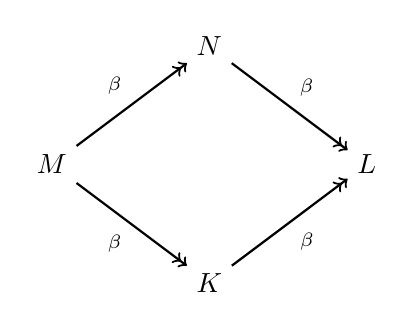
\begin{tikzpicture}[
    node distance=3cm,
    surj/.style={->>, line width=0.8pt}
    ]
    
    \node (M) at (0,0) {\(M\)};
    \node (N) at (2,1.5) {\(N\)};
    \node (K) at (2,-1.5) {\(K\)};
    \node (L) at (4,0) {\(L\)};
        
    \draw[surj] (M) -- node[above left]{\(\scriptstyle \beta\)} (N);
    \draw[surj] (M) -- node[below left]{\(\scriptstyle \beta\)} (K);
    \draw[surj] (N) -- node[above right]{\(\scriptstyle \beta\)} (L);
    \draw[surj] (K) -- node[below right]{\(\scriptstyle \beta\)} (L);
    
\end{tikzpicture}